% Standalone TikZ figure: Sim-to-Real Transfer Pipeline
% For Chapter 6: Domain Adaptation and Sim-to-Real Transfer
\documentclass[tikz,border=10pt]{standalone}
\usepackage{tikz}
\usepackage{amsmath}
\usetikzlibrary{arrows.meta, positioning, shapes.geometric, fit, backgrounds, calc, patterns, decorations.pathreplacing}

\begin{document}
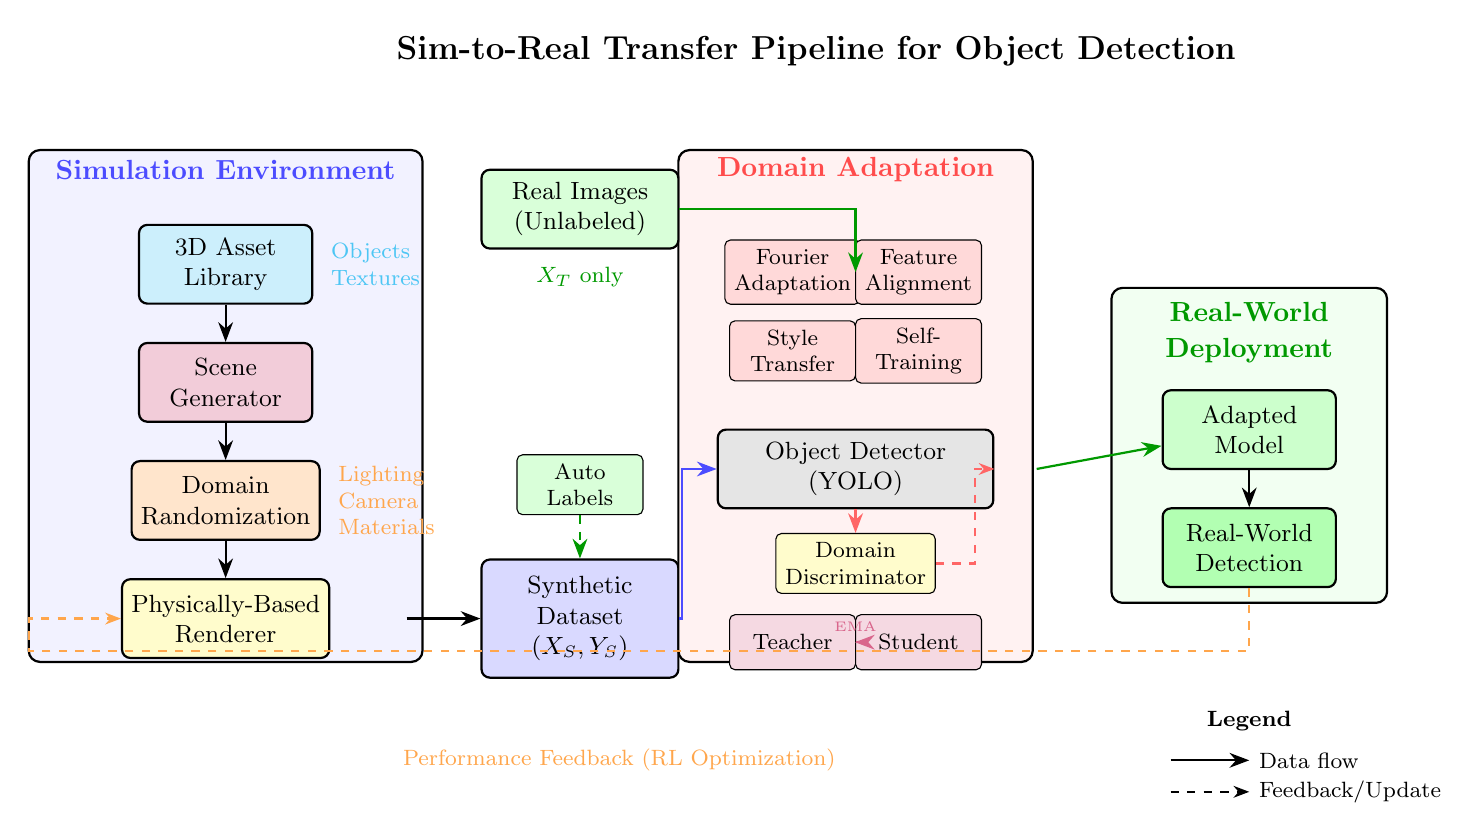
\begin{tikzpicture}[
    node distance=1cm and 1.5cm,
    every node/.style={font=\small},
    box/.style={rectangle, draw, thick, minimum width=2.2cm, minimum height=1cm, align=center, rounded corners=3pt},
    smallbox/.style={rectangle, draw, minimum width=1.6cm, minimum height=0.7cm, align=center, rounded corners=2pt, font=\footnotesize},
    arrow/.style={-{Stealth[length=2.5mm]}, thick},
    darrow/.style={-{Stealth[length=2mm]}, thick, dashed},
    label/.style={font=\footnotesize}
]

% Title
\node[font=\bfseries\large] at (7.5, 5) {Sim-to-Real Transfer Pipeline for Object Detection};

% ============ SIMULATION ENVIRONMENT ============
\begin{scope}[shift={(0, 0)}]
    % Background box
    \node[draw, thick, rounded corners, fill=blue!5, minimum width=5cm, minimum height=6.5cm] (simenv) at (0, 0.5) {};
    \node[font=\bfseries, blue!70] at (0, 3.5) {Simulation Environment};

    % 3D Assets
    \node[box, fill=cyan!20] (assets) at (0, 2.3) {3D Asset\\Library};

    % Scene Generator
    \node[box, fill=purple!20] (scenegen) at (0, 0.8) {Scene\\Generator};

    % Domain Randomization
    \node[box, fill=orange!20] (dr) at (0, -0.7) {Domain\\Randomization};

    % Renderer
    \node[box, fill=yellow!20] (render) at (0, -2.2) {Physically-Based\\Renderer};

    % Arrows within simulation
    \draw[arrow] (assets) -- (scenegen);
    \draw[arrow] (scenegen) -- (dr);
    \draw[arrow] (dr) -- (render);

    % Side annotations
    \node[label, right=0.1cm of assets, text=cyan!70, align=left] {Objects\\Textures};
    \node[label, right=0.1cm of dr, text=orange!70, align=left] {Lighting\\Camera\\Materials};
\end{scope}

% ============ SYNTHETIC DATA ============
\begin{scope}[shift={(4.5, -0.5)}]
    \node[box, fill=blue!15, minimum width=2.5cm, minimum height=1.5cm] (syndata) at (0, -1.7) {Synthetic\\Dataset\\$(X_S, Y_S)$};

    % Automatic labels annotation
    \node[smallbox, fill=green!15] (autolabel) at (0, 0) {Auto\\Labels};

    \draw[arrow] (-2.2, -1.7) -- (syndata);
    \draw[arrow, dashed, green!60!black] (autolabel) -- (syndata);
\end{scope}

% ============ DOMAIN ADAPTATION BLOCK ============
\begin{scope}[shift={(8, 0)}]
    % Background box
    \node[draw, thick, rounded corners, fill=red!5, minimum width=4.5cm, minimum height=6.5cm] (dablock) at (0, 0.5) {};
    \node[font=\bfseries, red!70] at (0, 3.5) {Domain Adaptation};

    % Methods
    \node[smallbox, fill=red!15] (fda) at (-0.8, 2.2) {Fourier\\Adaptation};
    \node[smallbox, fill=red!15] (feat) at (0.8, 2.2) {Feature\\Alignment};
    \node[smallbox, fill=red!15] (style) at (-0.8, 1.2) {Style\\Transfer};
    \node[smallbox, fill=red!15] (self) at (0.8, 1.2) {Self-\\Training};

    % Feature Extractor / Detector
    \node[box, fill=gray!20, minimum width=3.5cm] (detector) at (0, -0.3) {Object Detector\\(YOLO)};

    % Domain Discriminator
    \node[smallbox, fill=yellow!20] (disc) at (0, -1.5) {Domain\\Discriminator};

    % Adversarial training loop
    \draw[arrow, red!60] (detector) -- (disc);
    \draw[darrow, red!60] (disc.east) -- ++(0.5,0) |- (detector.east);

    % Teacher-Student
    \node[smallbox, fill=purple!15] (teacher) at (-0.8, -2.5) {Teacher};
    \node[smallbox, fill=purple!15] (student) at (0.8, -2.5) {Student};
    \draw[arrow, purple!60] (teacher) -- node[above, font=\tiny] {EMA} (student);
\end{scope}

% ============ REAL DATA (UNLABELED) ============
\begin{scope}[shift={(4.5, 3)}]
    \node[box, fill=green!15, minimum width=2.5cm, minimum height=1cm] (realdata) at (0, 0) {Real Images\\(Unlabeled)};
    \node[label, below=0.1cm of realdata, text=green!60!black] {$X_T$ only};
\end{scope}

% ============ DEPLOYMENT ============
\begin{scope}[shift={(13, 0.5)}]
    % Background box
    \node[draw, thick, rounded corners, fill=green!5, minimum width=3.5cm, minimum height=4cm] (deploy) at (0, -0.5) {};
    \node[font=\bfseries, green!60!black] at (0, 1.2) {Real-World};
    \node[font=\bfseries, green!60!black] at (0, 0.7) {Deployment};

    % Trained Model
    \node[box, fill=green!20] (model) at (0, -0.3) {Adapted\\Model};

    % Target Task
    \node[box, fill=green!30] (target) at (0, -1.8) {Real-World\\Detection};
\end{scope}

% ============ CONNECTING ARROWS ============
% Synthetic data to domain adaptation
\draw[arrow, blue!70] (syndata) -- ++(1.3,0) |- (detector);

% Real data to domain adaptation
\draw[arrow, green!60!black] (realdata) -| (8, 2.2);

% Domain adaptation to deployment
\draw[arrow, thick, green!60!black] (10.3, -0.3) -- (model);

% Model to target
\draw[arrow] (model) -- (target);

% ============ FEEDBACK LOOP ============
\draw[darrow, orange!70, thick] (target.south) -- ++(0,-0.8) -| (-2.5, -2.2) -- (render.west);
\node[label, orange!70, rotate=0] at (5, -4) {Performance Feedback (RL Optimization)};

% ============ LEGEND ============
\begin{scope}[shift={(13, -4)}]
    \node[font=\bfseries\footnotesize] at (0, 0.5) {Legend};
    \draw[arrow] (-1, 0) -- (0, 0);
    \node[label, right] at (0, 0) {Data flow};
    \draw[darrow] (-1, -0.4) -- (0, -0.4);
    \node[label, right] at (0, -0.4) {Feedback/Update};
\end{scope}

\end{tikzpicture}
\end{document}
